\section{Background}
John Maynard Keynes work revolutionized economic thought; however, he never formalized any of his theories into a mathematical theory. This was done over several decades in a process known as the Neo-classical synthesis which sought to connect traditional, classical models with newer Keynesian ideas\autocite{Fazzari1989}. In 1939, Paul Samuelson developed a popular model that could display endogenous, business-cycle behavior which married Keynes' investment multiplier theory with Clarke's accelerator principle\autocite{Puu2003,Press1939}.

The model is often criticized for the amount of simplifying assumptions it makes for the sake of mathematical simplicity. It is for this reason that later models feature significantly more mechanisms at play; however, this model is still useful for studying how cyclic behavior can be derived endogenously purely through economic fundamentals.
\subsection{Accelerator Theory and Investment}
Key to the idea of the accelerator effect is that growth has a positive effect on the level of investment. Economic growth features an overall increase in business profits and business confidence, thereby resulting in increases in fixed investments to grow business further. However, a recession decreases business profits and confidence and damages their ability and willingness to invest for the future. 

Earlier implementations of this theory used a simple, linear function to represent the relationship between investment and income. This however, was questioned on its applicability to real world behavior as it implied that business actively destroyed preexisting investments if income declined faster than the natural rate of capital depreciation. In the 1950s, Hicks suggested a linear, piecewise function with upper and lower bounds\autocite{Puu2003}. The lower bound represented the natural rate of capital depreciation thereby giving a minimal level of investment loss. The upper bound was rationalized to be a result of decreasing marginal gains to productivity from investment as land, labor, and raw materials became limiting factors to production. 

Richard Goodwin found a different solution in the form of a hyperbolic tangent function that asymptotically approached the limits of the piecewise function. This function was differentiable at all points which allows us to derive the form of the function used for our multiplier-accelerator model. Our investment function is a linear-cubic taylor series expansion of the hyperbolic tangent function which introduces a fundamental change in the function by causing it to backbend to 0 instead of asymptotically approaching a non-zero limit. This can be rationalized by introducing counter-cyclic government economic policy. During a recession, governments will increase spending in an attempt to counteract market behavior and stimulate the economy. Likewise, governments will take advantage of expansionary periods by increasing taxes and reducing government projects relative to recessionary periods allowing the government to possess the necessary funds to sustain investments come the next recessionary period. Our investment function can thus be thought of as being representative of both public and private investments.\autocite{Puu2003}

Investments are thus treated as a function of the change in income in the past with lag introduced, making it a second-order difference equation of the linear-cubic form:
\begin{equation}
    I_t=\mu(Y_{t-1}-Y_{t-2})-\mu(Y_{t-1}-Y_{t-2})^3
\end{equation}
\subsection{The Keynesian Multiplier and Consumption}
The Keynesian multiplier allows us to derive a relationship between income and the level of consumption. Much like investment, the model incorporates a lag into the reaction of consumption to income; however, this is now rationalized as a result of consumer's propensity to save and consume. This model holds propensity as a fixed parameter $s$ and sets propensity to consume as $1-s$. However, a key simplifying assumption made is by only allowing savings to last for a time period before being consumed. This is accomplished by the 2nd order difference equation:
\begin{equation}
    C_t=(1-s)Y_{t-1}+sY_{t-2}
\end{equation}
We can thus see that consumption is composed of two contributions, a 1-period delayed contribution due to the propensity to consume and a 2-period delayed contribution due to the propensity to save. 
\section{Stability and Chaos in Income Dynamics}
This economy does not store any income in an unproductive manner. Moreover, by effectively wrapping public investments in the cubic investment function and closing the economy from exports and imports, we reduce the outlets of income into two possible paths: consumption and investment.
\begin{equation}
    Y_t=C_t+I_t
\end{equation}
Incorporating our definitions of consumption and investment, we are able solve for future change in income as a function of previous change in income:
\begin{equation*}
    Y_t-Y_{t-1}=(\nu-s)(Y_{t-1}-Y_{t-2})-\nu(Y_{t-1}-Y_{t-2})^3
\end{equation*}
As we are most directly concerned with change in income, we can define a new variable:
\begin{equation*}
    Y_t-Y_{t-1}=Z_{t-1}
\end{equation*}
Thereby allowing us to simplify change in income to a first order difference equation:
\begin{equation}
    Z_t=\mu Z_{t-1}-(\mu+1)Z_{t-1}^3|\mu=\nu-s
\end{equation}

This is achieved due to a key economic feature of our parameter $\nu$. The value of $\nu$ is dependent on the choice of measure of income, it is thus linearly scalable which allows the model to be rescaled to this new parameter $\mu$ as this rescaling has no effect on the linear term. 

This rescaling allows us to significantly simplify analysis of the model as forces the model to pass through the points (0,0), (-1,1), and (1,-1).

Solving for fixed points, we have the trivial point $Z=0$; however, there also exists two non-origin points:
\begin{equation*}
    Z=\pm\sqrt{\frac{\mu-1}{\mu+1}}
\end{equation*}
Both of these points are stable in the region $0<\mu<2$ such that a positive initial value will tend towards the positive the positive fixed point while a negative initial value will tend towards the negative fixed point. This can be interpreted as having the economy face steady growth or decay ad infinitum which does not describe typical business cycle behavior.

Setting $\mu>2$, the fixed points lose stability and we then see the onset of stable cycles. However, it is important to note that these cycles feature oscillating levels of growth in the case of the positive domain or oscillating levels of decay in the negative domain. As the cycles do not oscillate between the positive and negative domains, the economy will still always either grow or decay depending on its initial state and parameter

\begin{figure}
    \centering
    \includegraphics[width=\textwidth]{./sam_hicks/2-cyclic.pdf}
    \caption{Cyclic growth behavior in the multiplier-accelerator model. As $Z>0$ for all iterations, the economy is perpetually growing albeit at an unsteady rate.}
\end{figure}
The feigenbaum point of this map occurs when $\mu\sim2.402$ which indicates the boundary point where chaos dominates the mapping. However, the chaotic behavior is still bounded in in one quadrant over successive iterations.
\begin{figure}
    \centering
    \includegraphics[width=\textwidth]{./sam_hicks/chaos_contained.pdf}
    \caption{Chaotic behavior in the multiplier-accelerator model contained in the positive quadrant.}
\end{figure}
Solving for the parameter value such that the maximal of the mapping is also the zero of the function allows us to define the boundary where the mapping's behavior is no longer bounded over successive iterations. The maximal of this mapping occurs at:
\begin{equation*}
    Z=\pm\frac{1}{\sqrt 3}\sqrt{\frac{mu}{\mu+1}}
\end{equation*}
This is equivalent to the zero of the mapping when 
\begin{equation*}
    \mu=\frac{3\sqrt{3}}{2}\sim2.5981
\end{equation*}
This point marks when the economy can begin actually facing cyclic growth and decay; however, as the behavior of the mapping is chaotic for most of this region, it does not feature regular shifts between growth and decay.

However, chaotic regions often features windows of order as is the case of this particular mapping when $\mu=2.7$ which features a stable, attractive cycle of 6 periodicity that is still able to feature growth and decay.
\begin{figure}
    \centering
    \includegraphics[width=\textwidth]{./sam_hicks/unbound_cyclic.pdf}
    \caption{Stable 6-period cycle in the multiplier-accelerator model featuring growth and decay.}
\end{figure}
Setting $\mu>3$ sees the model explode as the maximum exceeds the box set. This features unstable levels of extremely high magnitude growth and decay after a few relatively few iterations and is thus seen of little use in terms of applying to real-world business cycle dynamics.
\begin{figure}
    \centering
    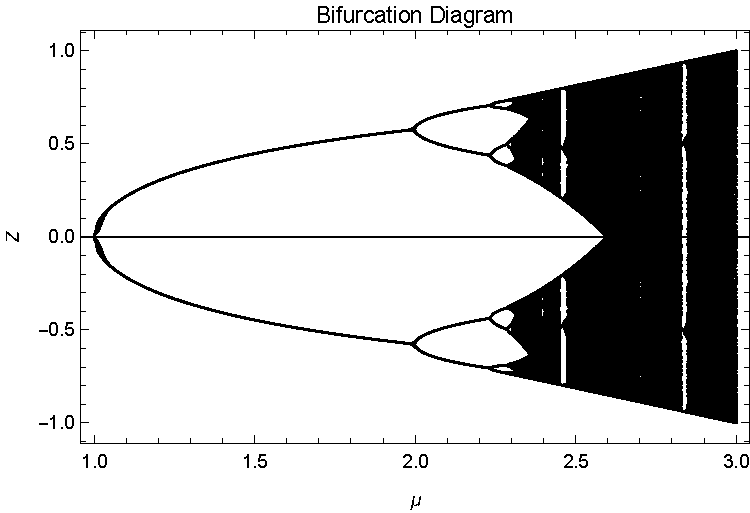
\includegraphics[width=\textwidth]{./sam_hicks/bifurcation.pdf}
    \caption{Bifurcation diagram of multiplier accelerator model. Black denotes plot with an initial value of 0.1, blue denotes plot with an initial value of -0.1. Convergence point denotes parameter value such that mapping can cross between quadrants.}
\end{figure}
\begin{figure}
    \centering
    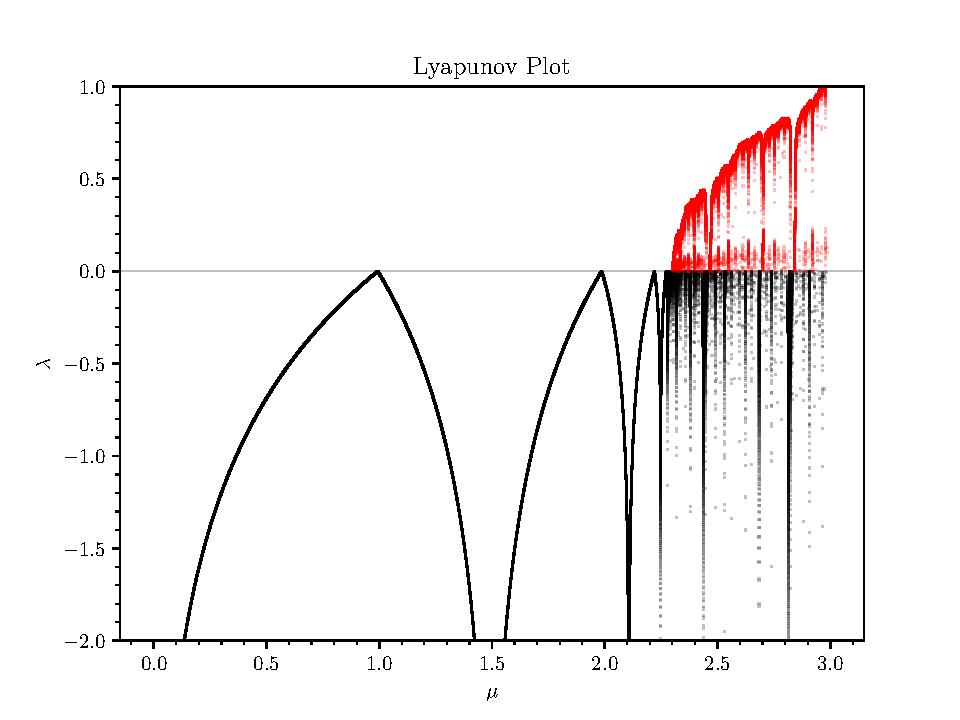
\includegraphics[width=\textwidth]{./sam_hicks/lyapunov.pdf}
    \caption{Lyapunov exponent plotted against $\mu$ for the samuelson-hicks. Initial value set to 0.1. Red denotes regions where $\lambda\geq0$, black denotes regions where $\lambda<0$}
\end{figure}